\documentclass[11pt,fleqn,twoside,a4paper]{article}
\usepackage{extsizes}
\usepackage[utf8]{inputenc}
\usepackage[T1]{fontenc}
\usepackage[left=40mm, right=40mm, top=35mm, bottom=35mm]{geometry}
\usepackage[ngerman]{babel}
\usepackage{amsmath,mathtools}
\usepackage{dsfont}
\usepackage{float}
\usepackage{multicol}
\usepackage{times}
\linespread{1.15}\selectfont
\usepackage[hang,footnotesize]{caption}

\usepackage{fancyhdr}
\fancypagestyle{titlestyle}{
  \fancyhf{}
  \renewcommand{\headrulewidth}{0pt}
  \renewcommand{\footrulewidth}{0pt}
}

\fancypagestyle{titleheadstyle}{
  \fancyhf{}
  \fancyfoot[C]{\footnotesize\bigskip\thepage}
  \renewcommand{\footrulewidth}{0.5pt}
  \renewcommand{\headrulewidth}{0pt}
}

\fancypagestyle{mainstyle}{
  \fancyhf{}
  \fancyfoot[C]{\footnotesize\bigskip\thepage}
  \fancyhead[RO]{\footnotesize \leftmark} %left
  \fancyhead[LE]{\footnotesize \leftmark} %right
  \renewcommand{\footrulewidth}{0.5pt}
  \renewcommand{\headrulewidth}{0.5pt}
}

\pagestyle{mainstyle}

\usepackage{titlesec}
\titleformat*{\section}{\large\bfseries}
\titleformat*{\subsection}{\bfseries}
\titleformat*{\subsubsection}{\bfseries}


\usepackage[dvipsnames]{xcolor}
\usepackage{listings}
\usepackage{tcolorbox}
\tcbuselibrary{many}
\tcbset{fonttitle=\footnotesize}
\allowdisplaybreaks

% definitions for listing colors
\definecolor{codeDarkGray}{gray}{0.2}
\definecolor{codeGray}{gray}{0.4}
\definecolor{codeLightGray}{rgb}{0.94,0.94,0.91}
\definecolor{codeBorder}{rgb}{0.34,0.24,0.21}
% predefinitions for listings
\newcommand{\listingcall}{Listing}
\newlength{\listingframemargin}
\setlength{\listingframemargin}{1em}
\newlength{\listingmargin}
\setlength{\listingmargin}{0.08\textwidth}
% \newlength{\listingwidth}
% \setlength{\listingwidth}{ ( \textwidth - \listingmargin * \real{2} + \listingframemargin * \real{2} ) }
% definitions for list of listings
% \newcommand{\listoflistingscall}{\listingcall -Verzeichnis}
% \newlistof{listings}{listinglist}{\listoflistingscall}
% style definition for standard code listings
\lstdefinestyle{std}{
  belowcaptionskip=0.5\baselineskip,
  breaklines=true,
  frameround=tttt,
  % frame=false,
  xleftmargin=0em,
  xrightmargin=0em,
  showstringspaces=false,
  showtabs=false,
  % tab=\smash{\rule[-.2\baselineskip]{.4pt}{\baselineskip}\kern.5em},
  basicstyle= \fontfamily{pcr}\selectfont\footnotesize\bfseries\scriptsize,
  keywordstyle= \bfseries\color{MidnightBlue}, %\color{codeDarkGray},
  commentstyle= \itshape\color{codeGray},
  identifierstyle=\color{codeDarkGray},
  stringstyle=\color{BurntOrange}, %\color{codeDarkGray},
  numberstyle=\tiny\ttfamily,
  % numbers=left,
  numbersep = 1em,
  % stepnumber = 1,
  % captionpos=t,
  tabsize=4,
  % backgroundcolor=\color{codebLightGray},
  rulecolor=\color{codeBorder},
  framexleftmargin=\listingframemargin,
  framexrightmargin=\listingframemargin
}

\usepackage{enumitem}
\usepackage{multirow}
\usepackage{emptypage}
\usepackage{url}
% \usepackage{wasysym}
\newcommand{\Earth}{{Erde}}
\usepackage[font=footnotesize]{subcaption}

\newcommand{\setNatural}{\mathds{N}}
\newcommand{\setReal}{\mathds{R}}
\newcommand{\function}[3]{#1\colon#2\to#3}
\newcommand{\norm}[1]{\|#1\|}
\newcommand{\abs}[1]{\left|#1\right|}
\newcommand{\separate}{,\quad}
\newcommand{\define}{\coloneqq}
\newcommand{\curveBrackets}[1]{\left(#1\right)}
\newcommand{\boxBrackets}[1]{\left[#1\right]}
\newcommand{\m}[1]{\mathrm{#1}}
\newcommand{\dotp}[2]{\left\langle#1,#2\right\rangle}

\begin{document}
  \newgeometry{left=42mm,right=42mm}
  \pagestyle{titlestyle}
  {\LARGE\bfseries \begin{center}{Projektbericht: $n$-Körper Simulation}\end{center}}
  \bigskip
  \begin{minipage}[t][][c]{0.45\textwidth}
    \raggedleft{Clemens Anschütz \\ clemens.anschuetz@uni-jena.de}
  \end{minipage}
  \hfill
  \begin{minipage}[t][][c]{0.45\textwidth}
    \raggedright{Markus Pawellek \\ markuspawellek@gmail.com}
  \end{minipage}
  \bigskip
  \begin{figure}[H]
    \center
    \includegraphics[height=3.0cm]{pictures/cover_image.jpg}
  \end{figure}
  \bigskip
  \hrule
  \medskip
  \begin{abstract}
    \itshape
    In dieser Arbeit beschäftigten wir uns mit der Entwicklung und Analyse eines Systems, welches dazu fähig ist das $n$-Körper-Problem für gegebene Anfangswerte zu simulieren und grafisch darzustellen.
Wir behandelten die Theorie des allgemeinen $n$-Körper-Problems, sowie die einiger Spezialfälle.
Außerdem implementierten wir diverse numerische Integratoren und verglichen diese auf der Basis ihrer Ergebnisse in Bezug auf ihre Stabilität, Genauigkeit und Berechnungsgeschwindigkeit.
  \end{abstract}
  \medskip
  \hrule
  \bigskip
  \tableofcontents
  \bigskip
  \bigskip
  \bigskip
  \cleardoublepage
  \restoregeometry

  \pagestyle{mainstyle}
  \setcounter{page}{1}
  \thispagestyle{titleheadstyle}
  {\LARGE\bfseries \begin{center}{Projektbericht: $n$-Körper Simulation}\end{center}}
\bigskip
\begin{minipage}[t][][c]{0.45\textwidth}
  \raggedleft{Clemens Anschütz \\ clemens.anschuetz@uni-jena.de}
\end{minipage}
\hfill
\begin{minipage}[t][][c]{0.45\textwidth}
  \raggedright{Markus Pawellek \\ markuspawellek@gmail.com}
\end{minipage}
\bigskip
% \begin{figure}[H]
%   \center
%   \includegraphics[height=3.0cm]{pictures/cover_image.jpg}
% \end{figure}
\bigskip
\hrule
\medskip
\begin{abstract}
  \itshape
  In dieser Arbeit beschäftigten wir uns mit der Entwicklung und Analyse eines Systems, welches dazu fähig ist das $n$-Körper-Problem für gegebene Anfangswerte zu simulieren und grafisch darzustellen.
Wir behandelten die Theorie des allgemeinen $n$-Körper-Problems, sowie die einiger Spezialfälle.
Außerdem implementierten wir diverse numerische Integratoren und verglichen diese auf der Basis ihrer Ergebnisse in Bezug auf ihre Stabilität, Genauigkeit und Berechnungsgeschwindigkeit.
\end{abstract}
\medskip
\hrule
\bigskip
\bigskip
  % \begin{multicols}{2}
    \section{Einleitung} % (fold)
\label{sec:einleitung}

  In der Physik und Mathematik ist es häufig so, dass realistisch modellierte Problemstellungen zu Differentialgleichungssystemen führen, die im allgemeinen nicht mehr analytisch lösbar sind.
  Um dennoch das Verhalten solcher Systeme näherungsweise beschreiben zu können, bildeten sich im Laufe der Zeit verschiedene Approximationsverfahren heraus.
  Darunter sind Verfahren, welche schwache Effekte mit geringer Auswirkung ignorieren und so die Problemstellung bis zu einem Punkt vereinfachen, an dem diese eine analytische Lösung besitzt.
  Andere Verfahren bauen auf dieser Methode auf und versuchen durch die Anwendung von Störungstheorie die schwachen Effekte im Nachhinein in die Lösung des vereinfachten Problems mit einzubauen.
  Ein Nachteil dieser Herangehensweise besteht jedoch darin, dass die Gleichungen, die eine Approximation der Lösung beschreiben, immer komplizierter werden, je mehr Effekte in die Störung mit einbezogen werden.
  Unter Umständen kann es sogar sein, dass gewisse Näherungen nur für spezielle Fälle des eigentlichen Problems ihre Gültigkeit behalten.
  Demzufolge ist es für die genannten Verfahren praktisch gesehen nicht möglich, die allgemeine Lösung solch komplexer Probleme anzunähern.
  Heutzutage spielen genau aus diesen Gründen Computersimulationen eine große Rolle.
  Durch ihre enorme Berechnungsgeschwindigkeit ermöglichen sie es, komplizierte Problemstellungen mit vergleichsweise einfachen Methoden zu behandeln.

  Analoges gilt auch für das $n$-Körper-Problem.
  Schon für das Dreikörperproblem findet sich keine allgemeine geschlossene Lösung mehr.
  Auch das eingeschränkte Dreikörperproblem lässt sich nur näherungsweise durch die Anwendung von Störungstheorie beschreiben.
  Eine $n$-Körper-Simulation ist dagegen in der Lage für ein beliebiges $n\in\setNatural$ und beliebige Anfangswerte eine genäherte Lösung zu generieren, sofern die zugrundeliegende Hardware die nötigen Resourcen zur Verfügung stellen kann und mit der Software zusammenpasst.
  Eines der besten Beispiele ist wahrscheinlich die Milleniums-Simulation, wie sie in Abbildung \ref{fig:millenium} zu sehen ist.

  Das Problem bei Simulationen besteht allerdings darin, dass der Computer deterministisch ist und deswegen kleine Rechenfehler begeht, die sich sogar mit der Zeit verstärken können.
  Des Weiteren ist es einem Computer nur möglich Lösungen an endlich vielen Punkten auszuwerten.
  Eine Simulation muss aus diesen Gründen nicht nur wohlbedacht designet und implementiert werden, sondern auch auf ihre Validität überprüft werden.
  Bei falscher Handhabung kann dies dazu führen, dass die Aussage einer Simulation keinen Wert hat.

  In dieser Arbeit beschäftigen wir uns mit der Entwicklung und Analyse eines Systems, welches dazu fähig ist das $n$-Körper-Problem für gegebene Anfangswerte zu simulieren und grafisch darzustellen.
  Wir behandeln die Theorie des allgemeinen $n$-Körper-Problems, sowie die einiger Spezialfälle.
  Außerdem implementieren wir diverse numerische Integratoren und vergleichen diese auf der Basis ihrer Ergebnisse in Bezug auf ihre Stabilität, Genauigkeit und Berechnungsgeschwindigkeit.

  \urldef{\milleniumurl}\url{https://wwwmpa.mpa-garching.mpg.de/galform/virgo/millennium/galseq_D_063.jpg}
  \begin{figure}[h]
    \center
    \includegraphics[width=0.95\textwidth]{pictures/millenium.jpg}
    \caption{Die Abbildung zeigt eine grafische Ausgabe der Milleniums-Simulation, welche versucht unser gesamtes Universum nachzustellen. Es wird deutlich, dass Galaxienhaufen auf großem Maßstab eine netzartigen Struktur bilden. Eine solche Aussage hätte man unmöglich nur durch theoretische Berechnungen treffen können. \\ Quelle: \\ \milleniumurl}
    \label{fig:millenium}
  \end{figure}

% section einleitung (end)
    \cleardoublepage
    \thispagestyle{titleheadstyle}
    \section{Physikalische Grundlagen} % (fold)
\label{sec:grundlagen}

  \subsection{Das $n$-Körper-Problem} % (fold)
  \label{sub:das_n_koerper_problem}

    Das $n$-Körper-Problem betrachtet in seiner allgemeinen Form eine feste Anzahl von Punktmassen, die sich in einem Inertialsystem aufgrund der zwischen ihnen herrschenden Gravitationskraft bewegen.

    \begin{figure}[h]
      \center
      \includegraphics[width=0.95\textwidth]{pictures/gravitational_force.pdf}
      \caption{Die Skizze zeigt die Wirkung der Newtonschen Gravitationskraft anhand zweier Beispielmassen. Die Kraft wirkt entlang der Verbindungslinie der Punktmassen.}
    \end{figure}

    Seien also $n\in\setNatural$ die Anzahl der Punktmassen, $m_i\in\setReal^+$ die Masse und $\function{r_i}{\setReal^+}{\setReal^3}$ die Kurve der $i.$~Punktmasse für alle $i\in\setNatural$ mit $i\leq n$.
    Nach dem zweiten Newtonschen Axiom und dem Newtonschen Gravitationsgesetz mit der Gravitationskonstanten $\gamma$ müssen die Kurven der Punktmassen den folgenden Differentialgleichungen  für alle $i\in\setNatural$ mit $i\leq n$ und alle $t\in\setReal^+$ gehorchen.
    \[
      m_i\ddot{r}_i(t) = \sum_{{j=1,\ j\neq i}}^n \gamma m_im_j \frac{r_j(t)-r_i(t)}{\norm{r_j(t)-r_i(t)}^3}
    \]
    Der Einfachheit halber definieren wir die Beschleunigung $a_i$ einer Punktmasse für alle $i\in\setNatural$ mit $i\leq n$.
    \[
      \function{a_i}{\setReal^{3n}}{\setReal^3}
      \separate
      a_i(r_1,\ldots,r_n)\define \sum_{{j=1,\ j\neq i}}^n \gamma m_j \frac{r_j-r_i}{\norm{r_j-r_i}^3}
    \]
    Für alle $i\in\setNatural$ mit $i\leq n$ vereinfachen sich dann die Differentialgleichungen zu der folgenden Form.
    \[
      \ddot{r}_i(t) = a_i(r_1(t),\ldots,r_n(t))
    \]

    Die Beschleunigung einer jeden Punktmasse hängt damit für jeden gegebenen Zeitpunkt vom gesamten Konfigurationsraum ab.
    Aus diesem Grund erscheint es sinnvoll die gesamte Problemstellung in den Konfigurationsraum zu überführen.
    Hierzu definieren wir als erstes die verallgemeinerte Kurve im Konfigurationsraum.
    \[
      \function{r}{\setReal^+}{\setReal^{3n}}
      \separate
      r(t)\define (r_1(t),\ldots,r_n(t))
    \]
    Der nächste Schritt besteht darin, eine verallgemeinerte Beschleunigung im Konfigurationsraum zu definieren.
    \[
      \function{a}{\setReal^{3n}}{\setReal^{3n}}
      \separate
      a\circ r(t) \define (a_1\circ r(t),\ldots,a_n\circ r(t))
    \]
    Mit diesen Definitionen lässt sich das Problem nun wie folgt für alle $t\in\setReal^+$ formulieren.
    \[
      \ddot{r}(t) = a\circ r(t)
    \]

    Bei dem gegebenen Gleichungssystem handelt es sich um ein gewöhnliches $3n$-dimensionales Differentialgleichungssystem zweiter Ordnung, welches sich, sofern $n\geq 3$, nur für sehr spezielle Fälle analytisch lösen lässt.
    Die später vorgestellten numerischen Integratoren zur Approximation der Lösung eines Anfangswertproblems sind jedoch nur für Differentialgleichungssysteme erster Ordnung anwendbar.
    Deshalb wollen wir zudem eine verallgemeinerte Geschwindigkeit im Konfigurationsraum einführen.
    \[
      \function{v}{\setReal^+}{\setReal^{3n}}
      \separate
      v\define \dot{r}
    \]
    Nach Definition muss damit auch die folgende Gleichung für alle $t\in\setReal^+$ erfüllt sein.
    \[
      \dot{v}(t) = a\circ r(t)
    \]
    Diese Beziehung machen wir uns zu Nutze, um das Problem in den Phasenraum zu überführen.
    Wir definieren eine verallgemeinerte Kurve im Phasenraum, welche zu jedem Zeitpunkt die Orte und Geschwindigkeiten aller Punktmassen beschreibt.
    \[
      \function{p}{\setReal^+}{\setReal^{6n}}
      \separate
      p(t) \define
      \begin{pmatrix}
        r(t) \\ v(t)
      \end{pmatrix}
    \]
    Wie vorher, benötigen wir auch eine verallgemeinerte Beschleunigung im Phasenraum.
    \[
      \function{f}{\setReal^{6n}}{\setReal^{6n}}
      \separate
      f\circ p(t)\define
      \begin{pmatrix}
        v(t) \\ a\circ r(t)
      \end{pmatrix}
    \]
    Aus den Definitionen von $p$ und $f$ folgt dann unmittelbar ein äquivalentes gewöhnliches $6n$-dimensionales Differentialgleichungssystem erster Ordnung in dem für alle $t\in\setReal^+$ das folgende gilt.
    \[
      \dot{p}(t) = f\circ p(t)
    \]

  % subsection das_ (end)

  \subsection{Das Zweikörperproblem} % (fold)
  \label{sub:das_zweikoerperproblem}

    Das Zweikörperproblem ist eine spezielle Form des $n$-Körper-Problems, in welchem $n=2$ gilt und damit nur zwei Punktmassen, die sich gegenseitig beeinflussen, betrachtet werden.
    Das resultierende System von Differentialgleichungen lässt sich analytisch lösen und stellt gerade aus diesem Grund eine Möglichkeit dar numerische Integratoren in Bezug auf ihre Stabilität, Genauigkeit und Geschwindigkeit zu quantifizieren.

    Die Lösung des Zweikörperproblems leitet sich aus dem Einkörperproblem ab, durch die Betrachtung des Schwerpunktsystems und der Einführung der reduzierten Masse.
    Im System selbst gilt die Energie- und Drehimpulserhaltung.
    \[
      E = T + U = \frac{m_1}{2}\norm{v_1}^2 + \frac{m_2}{2}\norm{v_2}^2 - \frac{\gamma m_1m_2}{\norm{r_1-r_2}} = \m{const}
    \]
    \[
      L = L_1 + L_2 = m_1r_1\times v_1 + m_2r_2\times v_2 = \m{const}
    \]
    Hierbei bezeichnet $E$ die Gesamtenergie, $T$ die kinetische Energie, $U$ die potentielle Energie, $L$ den Gesamtdrehimpuls, $L_1$ den Drehimpuls der ersten Punktmasse und $L_2$ den Drehimpuls der zweiten Punktmasse.
    Die Bewegung der Punktmassen findet in einer festen Ebene statt.
    In dieser Ebene kann die Kurve für jede Masse relativ zum Schwerpunkt in Polarkoordinaten unabhängig von der Zeit angegeben werden.
    Jede Bahn stellt einen Kegelschnitt dar.
    \[
      \function{\varrho}{[0,2\pi)}{\setReal^+}
      \separate
      \varrho(\varphi) \define \frac{p}{1+\varepsilon \cos \varphi}
    \]
    Dabei stellt $p$ den Halbparameter (hier ist nicht das Partikelsystem gemeint), $\varepsilon$ die Exzentrizität und $\mu$ die reduzierte Masse dar.
    \[
      p \define \frac{\norm{L}^2}{\gamma \mu^2(m_1+m_2)}
      \separate
      \varepsilon \define \sqrt{1 + \frac{2E\norm{L}^2}{\gamma^2(m_1+m_2)^2\mu^3}}
      \separate
      \mu \define \frac{m_1m_2}{m_1+m_2}
    \]

    Im Schwerpunktsystem beschreiben die Kurven der beiden Massen demanch entweder Ellipsen für $\varepsilon < 1$, Parabeln für $\varepsilon = 1$ oder Hyperbeln für $\varepsilon > 1$.
    Durch Transformation in ein Inertialsystem mit einer vorhandenen Relativgeschwindigkeit im Bezug zum Schwerpunkt, lassen sich bei gebunden Bewegungen auch Zykloiden beobachten.

  % subsection das_zweikörperproblem (end)

  \subsection{Bahnelemente} % (fold)
  \label{sub:bahnelemente}

    Ist die Lösung des Zweikörperproblems beschränkt beziehungsweise gebunden, so bewegen sich wie im vorigen Abschnitt erklärt, die beiden Punktmassen auf Ellipsen im Raum.
    Um die Bewegung einer Punktmasse zu beschreiben, sind, wie aus der theoretischen Mechanik bekannt, sechs Koordinaten notwendig.
    Im kartesischen Inertialsystem, indem auch das Problem formuliert wurde, charakterisieren drei dieser Koordinaten die Position und drei die Geschwindigkeit.
    Dieses System eignet sich für die numerische Simulation.

    In der Astronomie sind diese sechs Koordinaten aber schwer zu messen.
    Aus diesem Grund haben sich die sogenannten Bahnelemente etabliert, die im klassischen Fall ebenfalls durch sechs Parameter $(p,\varepsilon,i,\Omega,\omega,t)$ angegeben werden.
    Hierbei bezeichnet $p$ den Halbparameter, $e$ die Exzentrizität, $i$ die Inklination, $\Omega$ die Winkel des aufsteigenden Knotens, $\omega$ das Argument der Periapsis und $t$ den Zeitbezug.
    Sie beschreiben direkt die Lage und Form der Ellipsen im Raum und eignen sich gerade deshalb zur quantitativen Beschreibungen von Planetenbahnen.
    Zur Beschreibung von Planeten eines Sonnensystems wird statt $p$ auch oft die große Halbachse $a$ verwendet.
    In Abbildung \ref{fig:bahnelemente-scetch} ist noch einmal die Bedeutung einiger Bahnelemente skizziert.

    \urldef{\bahnelementeScetch}\url{https://de.wikipedia.org/wiki/Datei:BahnelementeEllipse.svg}
    \begin{figure}[h]
      \center
      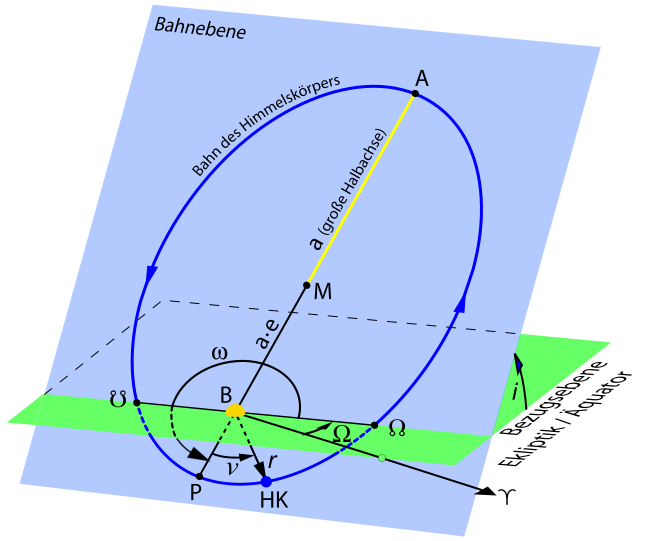
\includegraphics[width=0.95\textwidth]{pictures/BahnelementeEllipse.pdf}
      \caption{Die Skizze zeigt die Bedeutung der klassischen Bahnelemente. \\ Quelle:\\ \bahnelementeScetch}
      \label{fig:bahnelemente-scetch}
    \end{figure}
    Bei der quantitativen Auswertung der Simulation werden wir uns hauptsächlich auf die Parameter $\varepsilon$ und $a$ beziehen.
    Eine Formel zur Berechnung von $\varepsilon$ aus kartesischen Koordinaten wurde bereits in Abschnitt \ref{sub:das_zweikoerperproblem} genannt.
    Aus diesen Koordinaten kann ebenfalls $a$ berechnet werden.
    \[
      a = - \frac{\gamma\mu (m_1+m_2)}{2E}
      \separate
      \varepsilon \define \sqrt{1 + \frac{2E\norm{L}^2}{\gamma^2(m_1+m_2)^2\mu^3}}
    \]
    Die Berechnung der Inklination erfolgt meist über definition einer Bezugsebene, meist die Ekliptik.
    Wenn das Schwerpunktsystem so gewählt wurde, dass sich die Erde ausschließlich in der $xy$-Ebene bewegt, so kann die Inklination $i$ eines beliebigen Himmelskörpers, der den Drehimpuls $L$ besitzt einfach angebeben werden.
    \[
      i = \arcsin \curveBrackets{\frac{L_z}{\norm{L}}}
    \]

  % subsection bahnelemente (end)

  \subsection{Dreikörperproblem} % (fold)
  \label{sub:dreikörperproblem}

    Auch das Dreikörperproblem ist eine spezielle Form des $n$-Körper-Problems, in welchem $n=3$ gilt.
    Es ist im allgemeinen nicht mehr analytisch lösbar.
    Allerdings existieren geschlossene Lösungen für diverse Spezialfälle.
    In Abbildung \ref{fig:dreikoerper} sind beispielhafte Verläufe der Lösungen des Dreikörperproblems dargestellt.

    \urldef{\urldreikoerper}\url{https://tucschneider.files.wordpress.com/2015/03/dreikoerperproblem1.jpg}
    \urldef{\urlmotte}\url{http://scienceblogs.de/astrodicticum-simplex/2015/06/09/unloesbar-und-faszinierend-das-dreikoerperproblem/motte/}
    \begin{figure}[h]
      \center
      \begin{subfigure}{0.49\textwidth}
        \center
        \includegraphics[width=0.8\textwidth]{pictures/dreikoerperproblem1.jpg}
        % \caption{Typische Bahnkurven eines beliebig initialisierten Dreikörperproblems \\ Quelle: \urldreikoerper}
      \end{subfigure}
      \begin{subfigure}{0.49\textwidth}
        \center
        \includegraphics[width=0.8\textwidth]{pictures/motte.jpg}
        % \caption{Typische Bahnkurven eines beliebig initialisierten Dreikörperproblems \\ Quelle: \urldreikoerper}
      \end{subfigure}
      \caption{Die linke Abbildung zeigt die numerische Simulation eines Dreikörperproblems mit zufällig initialisierten Anfangswerten. Die rechte Abbildung zeigt eine spezielle analytische Lösung für die Bahnkurven des Dreikörperproblems. \\ Quellen: \\ \urldreikoerper \\ \urlmotte}
      \label{fig:dreikoerper}
    \end{figure}

  % subsection dreikörperproblem (end)

% section grundlagen (end)
    \cleardoublepage
    \thispagestyle{titleheadstyle}
    \section{Methoden und Implementierung} % (fold)
\label{sec:methoden_und_implementierung}

  \subsection{Programmstruktur} % (fold)
  \label{sub:strukturen}

    Das von uns erstellte Programm dient der numerischen Approximation von Lösungen des $n$-Körper-Problems für gegebene Anfangswerte.
    Um die Auswertung von Ergebnissen zu vereinfachen und intuitiver zu gestalten, implementierten wir neben den Integratoren eine graphische Ausgabe, eine einfache Form der Eingabe und diverse Möglichkeiten, um zwischen verschiedenen Einstellungen und Integratoren zur Laufzeit des Programmes zu wechseln.

    Bei der Ausgabe handelt es sich um eine perspektivische Projektion des betrachteten Raums auf den Bildschirm einer virtuellen Kamera.
    Position und Ausrichtung der Kamera lassen sich durch Mausinteraktionen beliebig einstellen.
    Zur Orientierung und Größeneinschätzung wird das Gitter eines Würfels mit Kantenlänge $1$ im Koordinatenursprung gezeigt.
    Die Punktmassen werden durch Kugeln dargestellt, deren Radien entsprechend ihrer Masse und ihres Abstandes zur Kamera skaliert werden.
    % Bananen waren keine gute Idee.
    Um die zurückgelegten Kurven der Partikel zu visualisieren, speicherten wir eine feste Anzahl von Bahnpunkten und verbanden diese durch Strecken.
    Das Tracken der Bahnpunkte erfolgte nicht nach jedem Zeitschritt, sondern wurde durch ein Kriterium festgelegt, welches sicher stellte, dass nur Punkte festgehalten wurden, die eine signifikante Richtungsänderung der Kurve hervorriefen.
    In Abbildung \ref{fig:program_example} werden die angegebenen Methoden noch einmal anhand eines Beispiels demonstriert.

    \begin{figure}[h]
      \center
      \includegraphics[width=0.95\textwidth]{pictures/program_example.jpg}
      \caption{Die Abbildung zeigt die Ausgabe des Programmes unter Verwendung des Sonnensystems als Beispielszenario. Zu erkennen sind unterschiedlich große Punktmassen und deren Bahnkurven. Das gezeigte Würfelgitter besitzt eine Kantenlänge von $1$.}
      \label{fig:program_example}
    \end{figure}

    Um die noch folgenden Integratoren zu verstehen und implementieren zu können, muss im Vorfeld über eine feste Datenstruktur, welche beschreibt, wie Positionen, Geschwindigkeiten und Massen der einzelnen Partikel zu speichern sind, entschieden werden.
    Zwei typische Varianten für eine solche Datenstruktur werden mit AOS (Array-of-Structure) und SOA (Structure-of-Array) bezeichnet.
    Im Folgenden sind für diese beiden Fälle einfache C++-Quelltexte angegeben.
    In beiden Fällen werden auf die C++-Standardbibliothek und die Bibliothek Eigen zugegriffen.
    Im Programm legten wir uns auf die AOS-Datenstruktur fest, da sie intuitiver im Umgang ist.
    \medskip
    \begin{tcolorbox}[colframe=black,colbacktitle=white,coltitle=black, attach boxed title to top center={yshift=-2mm},enhanced, titlerule=0.1pt, boxrule=0.5pt, arc=5pt,title=Quelltext:\quad SOA-Partikelsystem-Datenstruktur, breakable]
      \lstinputlisting[style=std,language=c++]{code/particle_system_soa.h}
    \end{tcolorbox}
    % \medskip

    % \medskip
    \begin{tcolorbox}[colframe=black,colbacktitle=white,coltitle=black, attach boxed title to top center={yshift=-2mm},enhanced, titlerule=0.1pt, boxrule=0.5pt, arc=5pt,title=Quelltext:\quad AOS-Partikelsystem-Datenstruktur, breakable]
      \lstinputlisting[style=std,language=c++]{code/particle_system_aos.h}
    \end{tcolorbox}

  % subsection strukturen (end)

  \subsection{Berechnung der Beschleunigung} % (fold)
  \label{sub:berechnung_der_beschleunigung}

    Die Berechnung der Beschleunigung kann direkt mithilfe der Gleichung aus Abschnitt \ref{sub:das_n_koerper_problem} erfolgen, indem für ein gegebenen Index $i\in\setNatural$ mit $i\leq n$ über alle anderen Partikel iteriert wird.
    \[
      a_i(r_1,\ldots,r_n) = \sum_{{j=1,\ j\neq i}}^n \gamma m_j \frac{r_j-r_i}{\norm{r_j-r_i}^3}
    \]
    Um jedoch numerische Singularitäten zu vermeiden, führten wir einen Parameter $\varepsilon\in\setReal^+$ ein, der sicherstellt, dass der Nenner des Bruches stets größer Null ist.
    Die leicht variierte Beschleunigung $\tilde{a}$ kann für alle $i\in\setNatural$ mit $i\leq n$ mit der folgenden Gleichung berechnet werden.
    \[
      \tilde{a}_i(r_1,\ldots,r_n)\define \sum_{{j=1,\ j\neq i}}^n \gamma m_j \frac{r_j-r_i}{\norm{r_j-r_i}^3 + \varepsilon}
    \]
    Zu beachten ist, dass durch die Einführung von $\varepsilon$ die Beschleunigung, die eine Punktmasse durch sich selbst erfährt, jetzt definiert und stets Null ist.
    \[
      \tilde{a}_i(r_1,\ldots,r_n) = \sum_{{j=1}}^n \gamma m_j \frac{r_j-r_i}{\norm{r_j-r_i}^3 + \varepsilon}
    \]
    Aus diesem Grund kann eine if-Abfrage für $i\neq j$ im Quelltext entfallen.
    Dies steigert das Optimierungspotential des Compilers und damit auch die resultierende Effizienz und Berechnungsgeschwindigkeit.
    Eine beispielhafte Implementierung in C++ ist im folgenden Quellcode gezeigt.

    \medskip
    \begin{tcolorbox}[colframe=black,colbacktitle=white,coltitle=black, attach boxed title to top center={yshift=-2mm},enhanced, titlerule=0.1pt, boxrule=0.5pt, arc=5pt,title=Quelltext:\quad Partikel-Beschleunigung, breakable]
      \lstinputlisting[style=std,language=c++]{code/particle_acceleration.cc}
    \end{tcolorbox}

  % subsection berechnung_der_beschleunigung (end)

  \subsection{Integratoren} % (fold)
  \label{sub:integratoren}

    Integratoren oder auch numerische Integratoren bezeichnen in der numerischen Mathematik Algorithmen, die entweder den Wert eines bestimmten Integrals oder die Lösung einer Differentialgleichung numerisch approximieren.
    Wir möchten uns hier auf die numerische Lösung von gewöhnlichen Differentialgleichungen beschränken.
    Integratoren werden immer dann verwendet, wenn analytische Lösungen nicht existieren oder zu kompliziert sind.
    In diesen Fällen reicht es aus, genäherte Lösungen mit beliebig kleinem Fehler zu bestimmen.

    Gerade beim $n$-Körper-Problem für $n\geq 3$ ist es demnach notwendig Integratoren zu verwenden, da allgemeine geschlossene Lösungen nicht existieren.
    Alle der hier verwendeten Integratoren lösen gewöhnliche Differentialgleichungssysteme erster Ordnung.
    Allerdings lässt sich das $n$-Körper-Problem wie in Abschnitt $\ref{sub:das_n_koerper_problem}$ gezeigt, in ein solches System überführen.

    Integratoren lassen sich nach ihrer Stabilität oder Robustheit, ihrer Genauigkeit und ihrer Geschwindigkeit einordnen.
    Die Geschwindigkeit ist durch eine einfache Zeitmessung bestimmbar.
    Um die Stabilität eines Integrators einzuschätzen, betrachten wir die Gesamtenergie des Systems, welche nach dem Energieerhaltungssatz konstant bleiben muss.
    Die Simulation eines analytisch lösbaren Problems, wie zum Beispiel des Zweikörperproblems, macht es zudem möglich die Genauigkeit eines Integrators zu bewerten.

    In den folgenden Abschnitten betrachten wir einige typische Integratoren, implementieren diese und schätzen sie nach den genannten Kriterien ein.
    Für $k\in\setNatural$ nennen wir $t_k\in\setReal^+$ den $k$.~Zeitpunkt mit der Bedingung $t_k < t_{k+1}$ für alle $k\in\setNatural$.
    Zudem nennen wir den $\Delta t \define t_{k+1}-t_k$ den Zeitschritt für äquidistante Zeitdiskretisierungen.
    Des Weiteren definieren wir $p_k$ als die numerische Approximation des gewählten Integrators von $p(t_k)$ für alle $k\in\setNatural$.

  % subsection integratoren (end)

  \subsection{Explizites Euler-Verfahren} % (fold)
  \label{sub:euler_verfahren}

    Das explizite Euler-Verfahren ist eines der simpelsten und intuitivsten Verfahren zur Approximation von gewöhnlichen Differentialgleichungen erster Ordnung.
    Dieses einfache Verfahren nähert die Zeitableitung in der Differentialgleichung durch den diskreten rechtsseitigen Differenzenquotient.
    Gemäß unserer Notation aus Abschnitt \ref{sub:das_n_koerper_problem} kann der explizite Euler-Algorithmus für alle $k \in \setNatural$ mit gegebenen Anfangswerten $p_1$ wie folgt aufgeschrieben werden.
    \[
      p_{k+1} = p_k + \Delta t \cdot f(p_k)
    \]
    Eine äquivalente Formulierung für die Kurven des Konfigurationsraumes ist im folgenden Gleichungssystem gegeben.
    \[
      \begin{pmatrix}
        r_{k+1} \\ v_{k+1}
      \end{pmatrix}
      \define
      \begin{pmatrix}
        r_k \\ v_k
      \end{pmatrix}
      + \Delta t \cdot
      \begin{pmatrix}
        v_k \\ a(r_k)
      \end{pmatrix}
    \]
    Das explizite Euler-Verfahren konvergiert in erster Ordnung mit dem Zeitschritt $\Delta t$.
    Im Allgemeinen erhält es nicht die Energie des betrachteten Systems.
    \medskip
    \begin{tcolorbox}[colframe=black,colbacktitle=white,coltitle=black, attach boxed title to top center={yshift=-2mm},enhanced, titlerule=0.1pt, boxrule=0.5pt, arc=5pt,title=Quelltext:\quad Expliziter Euler-Integrator, breakable]
      \lstinputlisting[style=std,language=c++]{code/euler_integrator.cc}
    \end{tcolorbox}

  % subsection euler_verfahren (end)

  \subsection{Symplektisches Euler-Verfahren} % (fold)
  \label{sub:symplektisches_euler_verfahren}

    Verfahren wie der explizite Euler, die keine Energieerhaltung aufweisen, neigen dazu nummerische Fahler in jedem Schritt aufzusummieren, wodurch die numerische Lösung mit der Zeit immer weiter von der analytischen weg driftet.
    Ein Lösungsansatz für dieses Problem sind symplektische Verfahren.
    Sie bestehen oft aus einer Mischung von expliziten und impliziten Methoden.
    Als einfachstes sei hier das semi-explizite Euler-Verfahren gezeigt.
    \[
      \begin{pmatrix}
        r_{k+1} \\ v_{k+1}
      \end{pmatrix}
      \define
      \begin{pmatrix}
        r_k \\ v_k
      \end{pmatrix}
      + \Delta t \cdot
      \begin{pmatrix}
        v_{k+1} \\ a(r_k)
      \end{pmatrix}
    \]
    In der Umsetzung muss darauf geachtet werden zuerst die zweite Zeile des Gleichungssystems zu berechnen, da diese die für die erste Zeile notwendige Geschwindigkeit $v_{k+1}$ liefert.
    Genau wie das explizite Euler-Verfahren konvergiert es in erster Ordnung.
    Im folgenden ist ein Codebeispiel gezeigt.
    \medskip
    \begin{tcolorbox}[colframe=black,colbacktitle=white,coltitle=black, attach boxed title to top center={yshift=-2mm},enhanced, titlerule=0.1pt, boxrule=0.5pt, arc=5pt,title=Quelltext:\quad Symplektischer Euler-Integrator, breakable]
      \lstinputlisting[style=std,language=c++]{code/symplectic_euler_integrator.cc}
    \end{tcolorbox}

  % subsection symplektisches_euler_verfahren (end)

  \subsection{Leapfrog-Verfahren} % (fold)
  \label{sub:leapfrog_verfahren}

    Ein weiteres symplektisches Verfahren ist das Leapfrog-Verfahren.
    Wie in den folgenden Gleichungen zu sehen, bezieht die Leapfrog-Methode auch Terme höherer Ordnung $\Delta t^2$ in die Integration mit ein.
    \[
      \begin{pmatrix}
        r_{k+1} \\ v_{k+1}
      \end{pmatrix}
      \define
      \begin{pmatrix}
        r_k \\ v_k
      \end{pmatrix}
      +
      \begin{pmatrix}
        v_k\Delta t + \frac{1}{2}a(r_k)\Delta t^2 \\
        \frac{1}{2}(a(r_k) + a(r_{k+1}))\Delta t
      \end{pmatrix}
    \]
    Das Verfahren konvergiert in zweiter Ordnung und ist damit präziser als die beiden zuvor eingeführten Euler-Verfahren.
    Die Implementierung kann wie im folgenden Beispiel gezeigt erfolgen.
    \medskip
    \begin{tcolorbox}[colframe=black,colbacktitle=white,coltitle=black, attach boxed title to top center={yshift=-2mm},enhanced, titlerule=0.1pt, boxrule=0.5pt, arc=5pt,title=Quelltext:\quad Leapfrog-Integrator, breakable]
      \lstinputlisting[style=std,language=c++]{code/leapfrog_integrator.cc}
    \end{tcolorbox}


  % subsection leapfrog_verfahren (end)

  \subsection{Runge-Kutta-Verfahren} % (fold)
  \label{sub:runge_kutta_verfahren}

    % Das Runge-Kutta-Verfahren ist nicht nur kompliziert auszusprechen und zu schreiben sondern auch noch hochgradig abstruse Alchemie und willkürliches Zusammenwerfen von unnachvollziehbaren Koeffizienten.
    Das klassische Runge-Kutta-Verfahren (RK4) ist ein nicht-symplektisches Integrationsverfahren, welches in vierter Ordnung konvergiert.
    Es ist eines der am häufigsten verwendeten Verfahren für gewöhnliche Differentialgleichungen.
    Die Idee des RK4 ist, in jedem Integrationsschritt die Ableitung an vier Punkten, dem Intervallanfangspunkt, zweimal in der Intervallmitte und dem Intervallendpunkt, abzuschätzen.
    Die Berechnung kann, wie in den folgenden Gleichungen dargestellt, erfolgen.
    \[
      p_{k+1} \define p_k + \frac{\Delta t}{6} \cdot (q_1 + 2q_2 + 2q_3 + q_4)
    \]
    \begin{align*}
      q_1 &\define f(p_k) & q_2 &\define f\curveBrackets{p_k + \frac{\Delta t}{2}q_1} \\
      q_3 &\define f\curveBrackets{p_k + \frac{\Delta t}{2}q_2} & q_4 &\define f\curveBrackets{p_k + \Delta t q_3}
    \end{align*}
    Es existieren neben dem RK4 auch noch weitere und allgemeinere Runge-Kutta-Verfahren für verschiedene Stufen und Konvergenzordnungen.
    Im Anschluss ist ein Beispielquelltext zur Implementierung des RK4 gezeigt.
    \medskip
    \begin{tcolorbox}[colframe=black,colbacktitle=white,coltitle=black, attach boxed title to top center={yshift=-2mm},enhanced, titlerule=0.1pt, boxrule=0.5pt, arc=5pt,title=Quelltext:\quad Runge-Kutta-Integrator, breakable]
      \lstinputlisting[style=std,language=c++]{code/runge_kutta_integrator.cc}
    \end{tcolorbox}

  % subsection runge_kutta_verfahren (end)

  \subsection{Adaptiver Zeitschritt} % (fold)
  \label{sub:adaptiver_zeitschritt}

    Bis jetzt wurde der Zeitschritt $\Delta t$ als Konstante betrachtet.
    Seine Verringerung führt zu genaueren Ergebnissen, steigert aber auch die benötigte Rechenzeit und den Rundungsfehler.
    Bei der manuellen Wahl der Schrittweite muss also immer im Vorhinein eine Abschätzung getroffen werden, um einerseits den Echtzeitaufwand erträglich zu halten, andererseits die numerischen Fehler nicht zu grob werden zu lassen.

    Betrachten wir ein typisches Sonnensystem mit einem massereichen Zentralgestirn, so sind die sonnennächsten Planeten besonders empfindlich gegenüber Erhöhungen des Zeitschritts, da sie die größte Änderung pro Iteration erfahren.
    Eine Möglichkeit zur Steuerung der Schrittweite besteht also in der Abschätzung der Umlaufzeit der schnellsten Punktmasse und entsprechender Unterteilung, zum Beispiel eine Schrittweite soll maximal ein tausendstel der Umlaufzeit des Merkurs betragen.
    Bei nicht hierarchischen $n$-Körper-Problemen ist eine solche Vorgehensweise nicht mehr unbedingt sinnvoll, manchmal auch nicht möglich, da sich unter Umständen keine Umlaufzeiten mehr definieren lassen.
    Aus diesem Grund haben wir uns bei der adaptiven Schrittweitensteuerung auf eine typische Methode gestützt.

    Zunächst erfolgt ein Integrationsschritt mit einfacher Schrittweite $\Delta t$, das Ergebnis wird beispielsweise als $p_{k+1}^{(1)}$ abgespeichert.
    \[
      p_k \xrightarrow{\Delta t} p_{k+1}^{(1)}
    \]
    Anschließend wird das ursprüngliche System $p_k$ zweimal jeweils über einen halben Zeitschritt propagiert und das somit berechnete Partikelsystem als $p_{k+1}^{(2)}$ gespeichert.
    \[
      p_k \xrightarrow{\frac{\Delta t}{2}} p_{k+\frac{1}{2}} \xrightarrow{\frac{\Delta t}{2}} p_{k+1}^{(2)}
    \]
    Als nächstes erfolgt die Berechnung des Residuums $\tau$.
    \[
      \tau \define p_{k+1}^{(2)} - p_{k+1}^{(1)}
    \]
    Falls die numerische Integration die exakte Lösung liefern würde, müsste $\tau = 0$ gelten.
    Je größer die Schrittweite, desto mehr weichen nun $p_{k+1}^{(1)}$ und $p_{k+1}^{(2)}$ voneinander ab.
    Zur Einschätzung, ob der Zeitschritt ausreichend klein gewählt wurde, kann nun eine Residuumsnorm von $\tau$ bestimmt werden.
    Um auch die Fehler einzelner Partikel nicht als Ausreißer zu betrachten, wählten wir nicht die Euklidische-Standardnorm, sondern die Maximumsnorm.
    \[
      \norm{\tau} = \max\left\{\abs{\tau_i} \ \middle| \ i\in\setNatural,i\leq 6n \right\}
    \]
    Die Anpassung des Zeitschrittes erfolgt dann nach der folgenden Formel, wobei $\delta\in\setReal^+$ die maximale Toleranz für den Fehler der Berechnung darstellt.
    \[
      \Delta t_{k+1} = 0.9\cdot\Delta t\cdot \min\curveBrackets{2,\max\curveBrackets{0.3, \frac{\delta}{\norm{\tau}}}}
    \]
    \medskip
    \begin{tcolorbox}[colframe=black,colbacktitle=white,coltitle=black, attach boxed title to top center={yshift=-2mm},enhanced, titlerule=0.1pt, boxrule=0.5pt, arc=5pt,title=Quelltext:\quad Adaptiver-Integrator, breakable]
      \lstinputlisting[style=std,language=c++]{code/adaptive_integrator.cc}
    \end{tcolorbox}


    % Der Zeitschritt kann nur über Userinteraktion erfolgen.

  % subsection adaptiver_zeitschritt (end)

  \subsection{Skalierung} % (fold)
  \label{sub:skalierung}

    Bei der numerischen Simulation physikalischer Problemstellungen ist es notwendig, eine geeignete Skalierung der physikalischen Größen zu implementieren oder festzulegen.
    Die effizienteste Möglichkeit besteht darin, direkt an der Schnittstelle zwischen Eingabe und Berechnung beziehungsweise zwischen Ausgabe und Berechnung gegebene Daten in eine feste Einheit umzuwandeln.
    Durch ein gut gewähltes Einheitensystem können numerische Rundungsfehler, die auf Gleitkommazahlen basieren, positiv beeinflusst werden.
    In den hier angegebenen Codebeispielen haben wir uns für die folgenden Einheiten entschieden.
    \begin{align*}
      [m] &= 1\,\m{M_{\Earth}} = 5.9722\cdot10^{24}\,\m{kg} \\
      [r] &= 1\,\m{AE} = 149597870700\,\m{m} \\
      [t] &= 1\,\m{a} = 31536000\,\m{s} \\
      [v] &= \frac{[r]}{[t]} = 4743.717361111\,\m{ms}^{-1}
    \end{align*}
    Durch Wahl dieses Systems muss nun auch die Gravitationskonstante im Newtonschen Gravitationsgesetz den Einheiten angepasst werden.
    Demzufolge ergibt sich der folgende Wert.
    \[
      \gamma = 6.674\cdot 10^{-11} \,\m{m^3\cdot kg^{-1}\cdot s^{-2}} =1.18406 \cdot 10^{-4} \,\m{AE^3\cdot M_\Earth^{-1}\cdot a^{-2}}
    \]
    % Das ist fast geil.

  % subsection skalierung (end)

% section methoden_und_implementierung (end)
    \cleardoublepage
    \thispagestyle{titleheadstyle}
    \section{Ergebnisse} % (fold)
\label{sec:ergebnisse}

  \subsection{Stabilitätsanalyse} % (fold)
  \label{sub:stabilitätsanalyse}

    Um die verschiedenen Integratoren auf ihre Genauigkeit und Stabilität hin zu untersuchen wurde ein bekanntes, analytisch lösbares Standardszenario simuliert, in diesem Fall das der Erde, die im Schwerefeld der Sonne kreist.
    Die Anfangswerte wurden dabei so gewählt, dass sie dem wirklichen Verlauf möglichst nahe kommen, so dass die Punktmasse Kreisbahnen um die Sonne beschreibt.
    Ein Integrator wird hier als stabil bezeichnet, wenn seine Lösungen beschränkt bleiben.
    Die Gesamtenergie des Systems erweist sich gutes Maß um die Stabilität einzuschätzen, da sie in gravitativ wechselwirkenden Systemen eine Erhaltungsgröße darstellt.
    Ist ein Integrator instabil, so wird sich die Gesamtenergie $E$ mit der Zeit verändern.
    Abbildung \ref{fig:sun_earth2} zeigt den Verlauf der Erdbahnkurve über mehrere Jahre für verschieden Integrationsmethoden.
    Wie man sieht, wächst die Lösung des expliziten Euler-Algorithmus mit jedem Integrationsschritt weiter an, der Planet entfernt sich immer weiter von der Sonne.
    Dieses Verhalten deckt sich gut mit der bekannten Charakteristik des Vorwärts-Euler-Integrators.
    Das Anwachsen der großen Halbachse ist mit einer Zunahme der Gesamtenergie verbunden, deren zeitliche Entwicklung in Diagramm \ref{fig:e2} dargestellt ist.
    Während die anderen Integratortypen vergleichsweise konstante Energiewerte über einen Zeitraum von $200\,\m{a}$ ausfweisen, steigt die des Euler-Integrators bereits in den ersten Jahren sehr stark an.
    Am Ende des betrachteten Bereichs geht $E$ langsam gegen Null, was einer ungebundenen Bewegung, beziehungsweise einer sehr großen Entfernung zum Stern entspricht.
    Ähnliches Verhalten ist auch beispielsweise bei der Berechnung des Federschwingers zu beobachten.

    Der symplektische Euler-Integrator weißt hingegen sehr wohl eine Energieerhaltung auf.
    Durch eine Kombination von implizitem und explizitem Algorithmus kann erreicht werden, dass sich die numerischen Fehler der beiden Methoden auf lange Sicht aufheben und die Bahnbewegung beschränkt bleibt.
    Die Breite der gezeigten Bahn weist darauf hin, dass jedoch sehr wohl numerische Ungenauigkeiten auftreten.
    Die Abweichungen verschiedener Umrundungen können von der grafischen Ausgabe nicht aufgelöst werden und erscheinen so als breitere Linien.

    \begin{figure}[p]
      \begin{subfigure}[b]{0.49\textwidth}
        \center
        \includegraphics[width=0.95\textwidth]{pictures/sun_earth/euler_0_02.jpg}
        \caption{Expliziter Euler-Integrator}
      \end{subfigure}
      \begin{subfigure}[b]{0.49\textwidth}
        \center
        \includegraphics[width=0.95\textwidth]{pictures/sun_earth/seuler_0_02.jpg}
        \caption{Symplektischer Euler-Integrator}
      \end{subfigure}

      \begin{subfigure}[b]{0.49\textwidth}
        \center
        \includegraphics[width=0.95\textwidth]{pictures/sun_earth/leapfrog_0_02.jpg}
        \caption{Leapfrog-Integrator}
      \end{subfigure}
      \begin{subfigure}[b]{0.49\textwidth}
        \center
        \includegraphics[width=0.95\textwidth]{pictures/sun_earth/rk4_0_02.jpg}
        \caption{RK4-Integrator}
      \end{subfigure}
      \caption{Die Abbildung zeigt den Verlauf der Bahnkurve der Erde in einem vereinfachten Sonne-Erde-System für verschiedene Integratoren mit einem Zeitschritt von $\Delta t = 0.020\,\m{a}$.}
      \label{fig:sun_earth2}
    \end{figure}

    \begin{figure}[p]
      \center
      \includegraphics[width=0.95\textwidth]{plots/sun_earth_2_plot.pdf}
      \caption{Das Diagramm zeigt die Entwicklung der Gesamtenergie $E$ im Verlauf der Simulations-Zeit $t$ für verschiedene Integratoren mit einem festen Zeitschritt $\Delta t = 0.020$.}
      \label{fig:e2}
    \end{figure}

    \begin{figure}[h]
      \center
      \includegraphics[width=0.95\textwidth]{plots/sun_earth_2_zoom_plot.pdf}
      \caption{Das Diagramm zeigt die Entwicklung der Gesamtenergie $E$ im Verlauf der Simulations-Zeit $t$ für verschiedene Integratoren mit einem festen Zeitschritt $\Delta t = 0.020$ und stellt zudem eine Vergrößerung des Diagrammes \ref{fig:e2} dar.}
      \label{fig:e2-zoom}
    \end{figure}

    In der grafischen Ausgabe sind die Unterschiede für einen kleineren Zeitschritt von $\Delta t = 0.02\,\m{a}$ zwischen Leapfrog- und dem RK4-Integrator nicht sichtbar.
    Beide erscheinen als perfekte Kreise und bestätigen die theoretischen Erwartungen.
    Allerdings sind in der Abbildung \ref{fig:e2-zoom}, die einen vergrößerten Bereich des Diagramms \ref{fig:e2} darstellt, durchaus geringe Unterschiede in beiden Verfahren erkennbar.
    Es wird deutlich, dass auch das Leapfrog-Verfahren Energieschwankungen aufweist, im Mittel dennoch die Energie erhält.
    Aufgrund der höheren Konvergenzordnung im Vergleich zum symplektischen Euler-Verfahren sind diese Schwankungen mehr als das zwanzigfache geringer.
    Das RK4-Verfahren arbeitet zwar mit einer Genauigkeit vierter Ordnung, ist aber nicht Energie-erhaltend.
    Wie in Abbildung \ref{fig:e2-zoom} zu erkennen, nimmt die Gesamtenergie über mehrere Iterationsschritte langsam ab, was bei einem expliziten Runge-Kutte-Integrator gerader Konvergenzordnung zu erwarten ist.
    Es muss sich demnach um ein instabiles Verfahren handeln.

    Die gezeigten Effekte werden durch die Wahl eines gröberen Zeitschrittes noch verstärkt.
    Abbildung \ref{fig:sun-earth-5} zeigt dasselbe Szenario für einen Zeitschritt von $\Delta t = 0.050\,\m{a}$.
    Das explizite Euler-Verfahren divergiert bereits nach einem fehlerhaften Umlauf.
    Die Instabilität des RK4-Verfahrens ist nun auch in der grafischen Ausgabe zu beobachten.
    Die Gesamtenergie nimmt im Laufe der Zeit ab, bis die Erde einen Minimalabstand zur Sonne unterschreitet und im darauffolgenden Integrationsschritt durch die Nähe zum Gravitationszentrum extrem beschleunigt wird und das System verlässt.
    Im Diagramm \ref{fig:e5} wird dieses Verhalten annähernd durch eine numerische Polstelle bei $t=200\,\m{a}$ beschrieben.
    Die beiden symplektischen Verfahren erhalten auch noch bei groben Zeitschritten die Gesamtenergie.
    In der grafischen Ausgabe äußern sich periodische Schwankungen der Energie durch periodische Schwankungen des Bahnradius.
    Die höhere Genauigkeit des Leapfrog-Verfahrens führt erneut zu einer Verringerung der Schwankungen gegenüber dem symplektischen Euler-Verfahren.

    \begin{figure}[p]
      \begin{subfigure}[b]{0.49\textwidth}
        \center
        \includegraphics[width=0.95\textwidth]{pictures/sun_earth/euler_0_05.jpg}
        \caption{Expliziter Euler-Integrator}
      \end{subfigure}
      \begin{subfigure}[b]{0.49\textwidth}
        \center
        \includegraphics[width=0.95\textwidth]{pictures/sun_earth/seuler_0_05.jpg}
        \caption{Symplektischer Euler-Integrator}
      \end{subfigure}

      \begin{subfigure}[b]{0.49\textwidth}
        \center
        \includegraphics[width=0.95\textwidth]{pictures/sun_earth/leapfrog_0_05.jpg}
        \caption{Leapfrog-Integrator}
      \end{subfigure}
      \begin{subfigure}[b]{0.49\textwidth}
        \center
        \includegraphics[width=0.95\textwidth]{pictures/sun_earth/rk4_0_05.jpg}
        \caption{RK4-Integrator}
      \end{subfigure}
      \caption{Die Abbildung zeigt den Verlauf der Bahnkurve der Erde in einem vereinfachten Sonne-Erde-System für verschiedene Integratoren mit einem Zeitschritt von $\Delta t = 0.050\,\m{a}$.}
      \label{fig:sun-earth-5}
    \end{figure}

    \begin{figure}[p]
      \center
      \includegraphics[width=0.95\textwidth]{plots/sun_earth_5_plot.pdf}
      \caption{Das Diagramm zeigt die Entwicklung der Gesamtenergie $E$ im Verlauf der Simulations-Zeit $t$ für verschiedene Integratoren mit einem festen Zeitschritt $\Delta t = 0.050$.}
      \label{fig:e5}
    \end{figure}

  % subsection stabilitätsanalyse (end)

  \subsection{Zweikörperproblem} % (fold)
  \label{sub:zweikörperproblem}

    Um die korrekte Funktionsweise der Integratoren zu überprüfen, haben wir, wie bereits in Abschnitt \ref{sub:das_zweikoerperproblem} erwähnt, analytisch lösbare Probleme simuliert.
    Vor allem das Zweikörperproblem stellt mit seiner Vielfalt an unterschiedlichen Lösungen eine ideale Testmöglichkeit dar.

    Die Lösungen des Zweikörperproblems teilen sich in gebundene und ungebundene Bewegungen ein.
    Abbildung \ref{fig:zkp-gebunden} zeigt diverse Beispiele dieser Bewegungen anhand eines Kreises, zweier sich nicht schneidender und zweier sich schneidender Ellipsen.
    Für das Szenario der konzentrischen Kreise in Abbildung \ref{subfig:konz-kreis} haben wir die Anfangswerte der beiden Massen so gesetzt, dass die Radialkräfte betragsmäßig gleich der Gravitationskraft zwischen beiden Punktmassen war.
    Den Schwerpunkt legten wir in den Koordinatenursprung.
    Für die beiden anderen Beispiele wählten kleinere Anfangsgeschwindigkeiten.
    \[
      m_1r_1 + m_2r_2 = 0
      \separate
      \frac{m_1\norm{v_1}^2}{\norm{r_1}} = \frac{\gamma m_1m_2}{\norm{r_1-r_2}^2} = \frac{m_2\norm{v_2}^2}{\norm{r_2}}
    \]
    \[
      \dotp{r_1}{v_1} = \dotp{r_2}{v_2} = 0
      \separate
      m_1v_1 + m_2v_2 = 0
    \]

    Die simulierten Partikelbahnen entsprechen somit den analytischen Lösungen und theoretischen Vorbetrachtungen.
    Dies spricht für die Genauigkeit der Integration.

    \begin{figure}
      \center
      \begin{subfigure}[b]{0.49\textwidth}
        \center
        \includegraphics[width=0.95\textwidth]{pictures/two_body/circle.jpg}
        \caption{konzentrische Kreise}
        \label{subfig:konz-kreis}
      \end{subfigure}
      \begin{subfigure}[b]{0.49\textwidth}
        \center
        \includegraphics[width=0.95\textwidth]{pictures/two_body/ellipse_no-intersect.jpg}
        \caption{nicht-schneidende Ellipsen}
      \end{subfigure}

      \begin{subfigure}[b]{\textwidth}
        \center
        \includegraphics[width=0.95\textwidth]{pictures/two_body/ellipse_intersect.jpg}
        \caption{schneidende Ellipsen}
      \end{subfigure}
      \caption{Die Abbildung zeigt Beispiele für gebundene Bahnkurven des Zweikörperproblems. Die Bahnen wurden mithilfe des adaptiven Leapfrog-Integrators simuliert.}
      \label{fig:zkp-gebunden}
    \end{figure}

    In Abbildung \ref{fig:zkp-zykloide} zeigen wir zudem ein Beispiel, in welchem das Inertialsystem nicht dem Schwerpunktsystem gleicht, sondern eine konstante Relativgeschwindigkeit zu diesem aufweist.
    Wie zu erwarten, sind sogenannte Taumelbewegungen oder auch Zykloiden zu beobachten.

    \begin{figure}[h]
      \center
      \includegraphics[width=0.95\textwidth]{pictures/two_body/cycloid.jpg}
      \caption{Die Abbildung zeigt ein Beispiel für eine gebundene Bahnkurven des Zweikörperproblems aus Sicht eines nicht im Schwerpunkt verankerten Inertialsystems. Es bilden sich typische Zykloide. Die Bahnen wurden mithilfe des adaptiven Leapfrog-Integrators simuliert.}
      \label{fig:zkp-zykloide}
    \end{figure}

    Die unbeschränkten Lösungen des Zweikörperproblems sind in den Beispielen in Abbildung \ref{fig:zkp-ungebunden} zu sehen.
    Man unterscheidet diese nach ihrer Exzentrizität $\varepsilon$.
    Für $\varepsilon = 1$ ergibt sich der Spezialfall einer Parabel, der erreicht werden kann, indem man die Anfangswerte der Punktmassen anpasst, sodass für die Gesamtenergie $E=0$ gilt.
    Für positive Energien ergeben sich Hyperbel-Bahnen, die sich im Unendlichen einer Gerade annähern.
    Alle genannten Eigenschaften konnten in unserer Simulation nicht nur qualitativ, sondern auch quantitativ bestätigt werden.

    \begin{figure}[h]
      \center
      \begin{subfigure}[b]{0.49\textwidth}
        \center
        \includegraphics[width=0.95\textwidth]{pictures/two_body/parabel.jpg}
        \caption{Parabel ($\varepsilon=1$)}
      \end{subfigure}
      \begin{subfigure}[b]{0.49\textwidth}
        \center
        \includegraphics[height=0.95\textwidth,angle=90]{pictures/two_body/hyperbol.jpg}
        \caption{Hyperbel ($\varepsilon >1$)}
      \end{subfigure}
      \caption{Die Abbildung zeigt Beispiele für nicht-gebundene Bahnkurven des Zweikörperproblems. Die Bahnen wurden mithilfe des adaptiven Leapfrog-Integrators simuliert.}
      \label{fig:zkp-ungebunden}
    \end{figure}

  % subsection zweikörperproblem (end)

  \subsection{Dreikörperproblem} % (fold)
  \label{sub:dreikörperproblem}

    Für das Dreikörperproblem gibt eine Vielzahl analytischer Lösungen für Spezialfälle.
    Wir wählten eine simplen Fall, bei dem die drei Punktmassen drei identische Kreisbahnen verfolgten.
    Dafür setzten wir die Anfangswerte der Massen, sodass der Betrag der Radialkraft jeder einzelnen Masse dem Betrag der Summe der Gravitationskräfte der übrigen Massen entsprach.
    Zudem positionierten wir die Punktmassen auf einem gleichseitigen Dreieck.

    In Abbildung \ref{fig:dkp} ist diese Anordnung und ihr zeitlicher Verlauf simuliert worden.
    Nach circa zweieinhalb Umdrehungen innerhalb von $7.5\,\m{a}$, die der geschlossenen Lösung entsprachen, begannen merkbare numerische Rundungsfehler zu erscheinen, wie sie bei $t=9.1\,\m{a}$ zu sehen sind.
    Diese verstärkten sich im folgenden Verlauf und führten zu immer größeren Asymmetrien.
    Nach fortgeschrittener Zeit erschien die Bewegung chaotisch.
    Wir schließen daraus, dass es sich bei dem berechneten Spezialfall nur um ein instabiles Gleichgewicht handeln kann.
    Kleinste Fehler, hier erzeugt durch Gleitkommaarithmetik, gleichen sich demnach nicht aus und divergieren.

    \begin{figure}[h]
      \center
      \begin{subfigure}[b]{0.49\textwidth}
        \center
        \includegraphics[width=0.95\textwidth]{pictures/three_body/triangle_1.jpg}
        \caption{$t=3.3\,\m{a}$}
      \end{subfigure}
      \begin{subfigure}[b]{0.49\textwidth}
        \center
        \includegraphics[width=0.95\textwidth]{pictures/three_body/triangle_2.jpg}
        \caption{$t=9.1\,\m{a}$}
      \end{subfigure}

      \begin{subfigure}[b]{0.49\textwidth}
        \center
        \includegraphics[width=0.95\textwidth]{pictures/three_body/triangle_3.jpg}
        \caption{$t=10.9\,\m{a}$}
      \end{subfigure}
      \begin{subfigure}[b]{0.49\textwidth}
        \center
        \includegraphics[width=0.95\textwidth]{pictures/three_body/triangle_4.jpg}
        \caption{$t=13.5\,\m{a}$}
      \end{subfigure}

      \begin{subfigure}[b]{0.49\textwidth}
        \center
        \includegraphics[width=0.95\textwidth]{pictures/three_body/triangle_5.jpg}
        \caption{$t=16.8\,\m{a}$}
      \end{subfigure}
      \begin{subfigure}[b]{0.49\textwidth}
        \center
        \includegraphics[width=0.95\textwidth]{pictures/three_body/triangle_6.jpg}
        \caption{$t=23.0\,\m{a}$}
      \end{subfigure}
      \caption{Die Abbildung zeigt den numerischen Verlauf der Bahnen eines Spezialfalls des Dreikörperproblems, dessen analytische Lösung drei identische Kreisbahnen wie im ersten Bild beschreibt. Die numerischen Fehler verstärken sich im Laufe der Zeit und führen somit zu chaotischen Bahnen. Es wurde das Leapfrog-Verfahren mit einem festen Zeitschritt von $\Delta t = 5\cdot 10^{-4}\,\m{a}$ verwendet.}
      \label{fig:dkp}
    \end{figure}

  % subsection dreikörperproblem (end)

  \subsection{Laufzeitanalyse} % (fold)
  \label{sub:laufzeitanalyse}

    Obwohl es beim Implementieren der Integratoren hauptsächlich um deren Stabilität und Genauigkeit ging, ist es für das spätere adaptive Zeitschrittverfahren relevant eine Performance-Analyse durchzuführen.
    Hierfür verwendeten wir für alle verfügbaren Integratoren ein System, bestehend aus $2000$ Punktmassen mit einer Zentralmasse.
    Die Berechnungsschritte pro Sekunde wurden vom Computer gemessen und ausgegen.
    Sie sind in Tabelle \ref{tab:fps} gegeben.

    \begin{table}[h]
      \caption{Die Tabelle zeigt die Iterationsschritte pro Sekunde (FPS) eines jeden Integrators, gemessen auf dem gleichen Computersystem, um diese miteinander zu vergleichen. Die Szene wurde durch $2000$ Punktmassen mit einer Zentralmasse beschrieben.}
      \label{tab:fps}
      \center
      \begin{tabular}{lcccc}
        \hline
        \hline
        Integrator & expliziter Euler & symplektischer Euler & Leapfrog & RK4 \\
        \hline
        FPS & $41$ & $41$ & $27$ & $17$ \\
        \hline
        \hline
      \end{tabular}
    \end{table}

    Wie zu erwarten, liefern die beiden Euler-Verfahren aufgrund ihrer ähnlichen und simplen Struktur, die maximale Performance unter den gemessenen Verfahren.
    Der Leapfrog-Integrator ist aufgrund seiner höheren Konvergenzordnung, welche einen komplizierteren Algorithmus zur Folge hat, langsamer.
    Analoges gilt für das RK4-Verfahren, welches algorithmisch gesehen das Aufwendigste der vewendeten Verfahren darstellt.

    Allerdings ist die Performance der Integratoren nicht ausschlaggebend, sobald sie zusammen mit einem adaptiven Zeitschrittverfahren verwendet werden.
    Es stellte sich heraus, dass für eine adaptive Wahl des Zeitschrittes ein Optimum aus Performance und Genauigkeit entscheidend war.
    So erschien das RK4-Verfahren trotz seines hohen Rechenaufwands dem expliziten Euler-Integrator weit überlegen, da die Schrittweitensteuerung wesentlich größere Zeitschritte verwendete.
    Die Zeit innerhalb der Simulation konnte somit schneller durchlaufen werden.

  % subsection laufzeitanalyse (end)

  \subsection{Simulation des Sonnensystems} % (fold)
  \label{sub:simulation_des_sonnensystems}

    Die absolute Kultaufgabe und Must-Have einer $n$-Körper-Simulation ist die Simulation des eigenen Sonnensystems.
    Deswegen widmeten auch wir uns dieser Aufgabe.
    Wir haben uns bewusst dazu entschieden, Pluto in die Planetensimulation mit einzubeziehen, da wir seine Ausgrenzung nicht unterstützen.
    Es sollte nicht immer auf die Größe ankommen.
    Für die Anfangswerte der Sonne und aller Planeten verwendeten wir bekannte Ephemeriden, siehe \ref{sec:ephemeriden_des_sonnensystem}.
    Ein beispielhafte grafische Ausgabe ist in Abbildung \ref{fig:solarsystem} gezeigt.
    Die Betrachtung dieser weckt heimatliche Gefühle.

    Um die Genauigkeit der Simulation anhand des Sonnensystems zu überprüfen, bestimmten wir die Mittelwerte diverser Kenngrößen aller Planeten im Sonnensystem.
    In Tabelle \ref{tab:solarsystem} sind diese Werte zusammen mit ihren bekannten Literaturwerten dargestellt.
    Der Vergleich mit den bekannten Literatur zeigt eine bemerkenswerte Übereinstimmung aller Werte.

    \begin{figure}[h]
      \center
      \begin{subfigure}[b]{0.49\textwidth}
        \center
        \includegraphics[width=0.95\textwidth]{pictures/solar_system/total.jpg}
        \caption{gesamtes Sonnensystem}
      \end{subfigure}
      \begin{subfigure}[b]{0.49\textwidth}
        \center
        \includegraphics[width=0.95\textwidth]{pictures/solar_system/zoom.jpg}
        \caption{innere Planetenbahnen}
      \end{subfigure}
      \caption{Die Abbildung zeigt eine Simulation des Sonnensystems basierend auf Ephemeriden. Die Berechnung erfolgten unter Verwendung des adaptiven Leapfrog-Verfahrens.}
      \label{fig:solarsystem}
    \end{figure}

    \urldef{\solarsystemdata}\url{https://de.wikipedia.org/wiki/Liste_der_Planeten_des_Sonnensystems}
    \urldef{\plutodata}\url{https://en.wikipedia.org/wiki/Pluto}
    \begin{table}[h]
      \center
      \caption{Die Tabelle zeigt simulierte und tabellarische Kennwerte der Planeten unseres Sonnensystems. Dabei bezeichnet $T$ die Umlaufzeit, $a$ die große Halbachse und $\varepsilon$ die Exzentrizität. Zugehörige Tabellenwerte sind durch den Index $\m{Tab}$ gekennzeichnet. \\ Quelle: \\ \solarsystemdata \\ \plutodata}
      \label{tab:solarsystem}
      \renewcommand{\arraystretch}{1.5}
      \begin{tabular}{l|rr|rr|rr}
        \hline
        Planeten & $T \ [\m{a}]$ & $T_\m{Tab}\ [\m{a}]$ & $a \ [\m{AE}]$ & $a_\m{Tab} \ [\m{AE}]$ & $\varepsilon$ & $\varepsilon_\m{Tab}$ \\
        \hline
        \hline
        Merkur & $0.241$ & $0.2410$ & $0.387$ & $0.387$ & $0.201$ & $0.206$ \\
        Venus & $0.616$ & $0.6156$ & $0.723$ & $0.723$ & $0.00639$ & $0.00677$ \\
        Erde & $1.001$ & $1.000$ & $0.999$ & $1.00$ & $0.0161$ & $0.0167$ \\
        Mars & $1.880$ & $1.882$ & $1.52$ & $1.52$ & $0.0939$ & $0.0934$ \\
        Jupiter & $11.85$ & $11.86$ & $5.20$ & $5.20$ & $0.0495$ & $0.0484$ \\
        Saturn & $29.40$ & $29.46$ & $9.56$ & $9.54$ & $0.0554$ & $0.0542$ \\
        Uranus & $84.07$ & $84.01$ & $19.2$ & $19.19$ & $0.0464$ & $0.0472$ \\
        Neptun & $164.9$ & $164.8$ & $30.1$ & $30.06$ & $0.00878$ & $0.00859$ \\
        Pluto & $247.9$ & $247.9$ & $39.6$ & $39.48$ & $0.250$ & $0.249$ \\
        \hline
        \hline
      \end{tabular}
    \end{table}

  % subsection simulation_des_sonnensystems (end)

  \subsection{Wahl des Zeitschrittes} % (fold)
  \label{sub:wahl_des_zeitschrittes}

    Komplizierte $n$-Körper-Probleme sind nicht nur aufwendig zu simulieren, sondern erfordern auch einen gut-gewählten Zeitschritt.
    Einen Zeitschritt im Vorfeld zu bestimmen, ist eine nicht-triviale Aufgabe und oft nicht praxistaugliches Verfahren.
    Das Setzen eines konstanten Zeitschrittes führt zudem notwendigerweise zu der Wahl einer sehr kleinen Schrittweite.
    Der Rechenaufwand und die damit benötigte Simulationszeit steigt damit erheblich, ohne sicher zu stellen, dass die Simulation in allen Schritten korrekt verläuft.
    Wie in Abschnitt \ref{sub:adaptiver_zeitschritt} beschrieben, konnten wir zeigen, dass die Wahl eines adaptiven Zeitschrittes überlegen zu den vorher genannten Methoden ist.
    Abbildung \ref{fig:20-koerper} stellt ein System von zwanzig Massen mit einem schweren Zentralkörper dar.
    Ein solches System benötigt je nach Anordnung und Zeitpunkt unterschiedliche Zeitschritte, da ansonsten die Bahnen der Planeten stark verfälscht werden, wie es in Abbildung \ref{subfig:20-koerper-konst} gezeigt ist.
    Der Zeitschritt war für einige der inneren Punktmassen zu grob gewählt und führte der Charakteristik des RK4-Verfahrens folgend zu Implosionen der Bahnen.
    Äußere Planeten zeigten jedoch keine sichtbaren Fehler und hätten mit einer noch größeren Schrittweite berechnet werden können.
    Durch Verwendung eines adaptiven Verfahrens konnten wir dergleichen verhindern.
    Abbildung zeigt \ref{subfig:20-koerper-adap} zeigt das gleiche System mit stabilen Bahnverläufen.
    Die gewählten Zeitschritte des Algorithmus lagen in dem Bereich $[0.0005\,\m{a},0.08\,\m{a}]$.
    Interessant ist dabei, dass der zuvor gewählte Zeitschritt innerhalb des gegebenen Intervalls liegt und nicht zu grob gewählt scheint.
    Dennoch scheinen kritische Zeitpunkte zu existieren, an denen die Wahl einer kleineren Schrittweite unerlässlich ist.
    Die Wahl einer Computer-gestützten Schrittweite sollte aus diesen Gründen der Wahl einer konstanten Schrittweise immer bevorzugt werden.

    \begin{figure}[h]
      \begin{subfigure}[b]{0.49\textwidth}
        \center
        \includegraphics[width=0.95\textwidth]{pictures/adaptive/shit.jpg}
        \caption{konstanter Zeitschritt $\Delta t = 0.070\,\m{a}$}
        \label{subfig:20-koerper-konst}
      \end{subfigure}
      \begin{subfigure}[b]{0.49\textwidth}
        \center
        \includegraphics[width=0.95\textwidth]{pictures/adaptive/good.jpg}
        \caption{adaptiver Zeitschritt}
        \label{subfig:20-koerper-adap}
      \end{subfigure}
      \caption{Die Abbildung zeigt eine $n$-Körper-Simulation mit $n=20$ für unterschiedliche Zeitschrittverfahren und einem RK4-Integrator. Das adaptive Verfahren zeigt keine divergierenden Bahnen im Gegensatz zur konstanten Zeitschrittwahl.}
      \label{fig:20-koerper}
    \end{figure}

  % subsection wahl_des_zeitschrittes (end)

  % \subsection{Vergleich mit Mercury6} % (fold)
  % \label{sub:vergleich_mit_mercury6}

  %   \begin{itemize}
  %     \item wahl eines einfachen systems
  %     \item vergleich der halbachse der erde
  %   \end{itemize}

  % subsection vergleich_mit_mercury6 (end)

% section ergebnisse (end)
    \cleardoublepage
    \thispagestyle{titleheadstyle}
    \section{Fazit} % (fold)
\label{sec:fazit}

  % Wir haben gut gearbeitet und denken, dass man uns fürstlich entlohnen sollte.
  Das Projekt diente dem Erstellen eines Programms zur numerischen Integration des $n$-Körper-Problems.
  Dazu wurden verschiedene Integrationsalgorithmen implementiert, Strukturen zur Beschreibung von Partikelsystemen erstellt, eine Ein- und Ausgaberoutine geschrieben, sowie eine grafische Oberfläche zur Visualisierung der Bahnverläufe und User-Interaktion programmiert.
  Wir wählten für das $n$-Körper-Problem typische Integrationsmethoden, wie das explizite Euler-, das symplektische Euler-, das Leapfrog- und das RK4-Verfahren, und verglichen diese.
  Um die Methoden hinsichtlich ihrer Stabilität zu überprüfen wurde das gut bekannte Szenario Erde im Schwerefeld der Sonne simuliert.
  Die Auswertung zeigte typische Eigenschaften der Integratoren auf.
  Das explizite Euler-Verfahren neigte als Integrator erster Ordnung zur stetigen Erhöhung der Energie und damit Bahnvergrößerung, während der RK4 als explizites Verfahren vierter Ordnung eine kontinuierliche Abnahme von Energie und Bahnradius zur Folge hatte.
  Die beiden symplektischen Verfahren verhielten sich aufgrund ihrer Energieerhaltung auch noch bei sehr groben Zeitschritten als außerordentlich robust.

  Im weiteren Verlauf wurde ein analytisch lösbares Dreikörperszenario simuliert.
  Es zeigte sich hierbei, dass die analytische Lösung keinesfalls ein stabiles Gleichgesicht beschrieb, weswegen kleinste numerische Ungenauigkeiten bereits nach wenigen Zyklen in chaotischem Verhalten resultierten.

  Die Simulation des Sonnensystems, sowie die etlicher bekannter Zweikörperprobleme lieferte Ergebnisse, die sich hervorragend mit den theoretischen Vorüberlegungen deckten. Somit bestätigte sich erneut die korrekte Arbeitsweise aller Integratoren.

  Bei der Analyse sehr großer Teilchensysteme erwies sich der Einsatz einer adaptiven Schrittweitensteuerung als wichtiger Garant für das Berechnen realistischer Bahnkurven.

  Zusammenfassend kann man sagen, dass die numerische $n$-Körpersimulation eine essenzielle Methode zur Berechnung und Analyse von Vielteilchensystemen darstellt.
  Für nicht-chaotische Systeme stellt es zudem eine Werkzeug zur Vorhersage dar, die weit außerhalb der Möglichkeiten analytischer Methoden liegen.



% section fazit (end)
    \cleardoublepage
    \thispagestyle{titleheadstyle}
    \section{Literatur} % (fold)
\label{sec:literatur}

	\begin{enumerate}[label=(\arabic*)]
		\item
		William M. Folkner, James G. Williams, Dale H. Boggs, Ryan S. Park, and Petr Kuchynka, \textit{The Planetary and Lunar Ephemerides DE430 and DE431}
		\item
		Pertsch: Skript Vorlesung Computational Physics
		\item
		\url{https://de.wikipedia.org/wiki/Bahnelement}
		\item
		\url{https://de.wikipedia.org/wiki/Zweikörperproblem}
		\item
		Walter Gautschi, \textit{Numerical Analysis}, zweite Auflage, Birkhäuser, 2012
		\item
		Ward Cheney, David Kingaid, \textit{Numerical Mathematics and Computing}, sechste Auflage, Thomson, 2008
		\item
		Wolfgang Nolting, \textit{Grundkurs Theoretische Physik 1: Klassische Mechanik}, neunte Auflage, Springer, 2011
		\item
		William H. Press, Saul A. Teukolsky, William T. Vetterling, Brian P. Flannery, \textit{Numerical Recipes in C: The Art of Scientific Computing}, zweite Auflage, Cambridge University Press, 2002
	\end{enumerate}

% section literatur (end)
    \cleardoublepage
    \thispagestyle{titleheadstyle}
    \appendix
    \pagenumbering{roman}
    \section{Ephemeriden des Sonnensystems} % (fold)
\label{sec:ephemeriden_des_sonnensystem}

  \begin{table}[h]
    \caption{Die Tabelle stellt die Anfangspositionen $r$, angegeben in Astronomischen Einheiten ($\m{AE}$), und -geschwindigkeiten $v$, angegeben in Astronomischen Einheiten pro Tag ($\m{AE}/\m{d}$), der Sonne und ihrer Planeten am 28.Juni 1969 in Bezug zum ICRF2-Koordinatensystem dar. \\ Quelle: [1]}
    \center
    \renewcommand{\arraystretch}{1.5}
    \scriptsize
    \begin{tabular}{llrrr}
      \hline
      \hline
      \multirow{2}{*}{Sun}
      & $r$ & 0.00450250878464055477 & 0.00076707642709100705 & 0.00026605791776697764 \\
      & $v$ & -0.00000035174953607552 & 0.00000517762640983341 & 0.00000222910217891203 \\
      \hline
      \multirow{2}{*}{Mercury}
      & $r$ & 0.36176271656028195477 & -0.09078197215676599295 & -0.08571497256275117236 \\
      & $v$ & 0.00336749397200575848 & 0.02489452055768343341 & 0.01294630040970409203 \\
      \hline
      \multirow{2}{*}{Venus}
      & $r$ & 0.61275194083507215477 & -0.34836536903362219295 & -0.19527828667594382236 \\
      & $v$ & 0.01095206842352823448 & 0.01561768426786768341 & 0.00633110570297786403 \\
      \hline
      \multirow{2}{*}{EM Bary}
      & $r$ & 0.12051741410138465477 & -0.92583847476914859295 & -0.40154022645315222236 \\
      & $v$ & 0.01681126830978379448 & 0.00174830923073434441 & 0.00075820289738312913 \\
      \hline
      \multirow{2}{*}{Mars}
      & $r$ & -0.11018607714879824523 & -1.32759945030298299295 & -0.60588914048429142236 \\
      & $v$ & 0.01448165305704756448 & 0.00024246307683646861 & -0.00028152072792433877 \\
      \hline
      \multirow{2}{*}{Jupiter}
      & $r$ & -5.37970676855393644523 & -0.83048132656339789295 & -0.22482887442656542236 \\
      & $v$ & 0.00109201259423733748 & -0.00651811661280738459 & -0.00282078276229867897 \\
      \hline
      \multirow{2}{*}{Saturn}
      & $r$ & 7.89439068290953155477 & 4.59647805517127300705 & 1.55869584283189997764 \\
      & $v$ & -0.00321755651650091552 & 0.00433581034174662541 & 0.00192864631686015503 \\
      \hline
      \multirow{2}{*}{Uranus}
      & $r$ & -18.26540225387235944523 & -1.16195541867586999295 & -0.25010605772133802236 \\
      & $v$ & 0.00022119039101561468 & -0.00376247500810884459 & -0.00165101502742994997 \\
      \hline
      \multirow{2}{*}{Neptune}
      & $r$ & -16.05503578023336944523 & -23.94219155985470899295 & -9.40015796880239402236 \\
      & $v$ & 0.00264276984798005548 & -0.00149831255054097759 & -0.00067904196080291327 \\
      \hline
      \multirow{2}{*}{Pluto}
      & $r$ & -30.48331376718383944523 & -0.87240555684104999295 & 8.91157617249954997764 \\
      & $v$ & 0.00032220737349778078 & -0.00314357639364532859 & -0.00107794975959731297 \\
      \hline
      \hline
    \end{tabular}
  \end{table}

% section ephemeriden_des_sonnensystem (end)
  % \end{multicols}
\end{document}